\documentclass[class=article,border=0pt]{standalone}

%------------------------------------------------------------------------------
%                         COLORS
%------------------------------------------------------------------------------
\usepackage{xcolor}

%------------------------------------------------------------------------------
%                          TIKZ
%------------------------------------------------------------------------------
\usepackage{tikz}

\tikzset{
	graphnode/.style = {align=center, inner sep=0pt, text centered, font=\sffamily},
	kmer/.style = {graphnode, circle, black, font=\sffamily\bfseries, draw=black, fill=white, text width=3em},
}

\begin{document}
	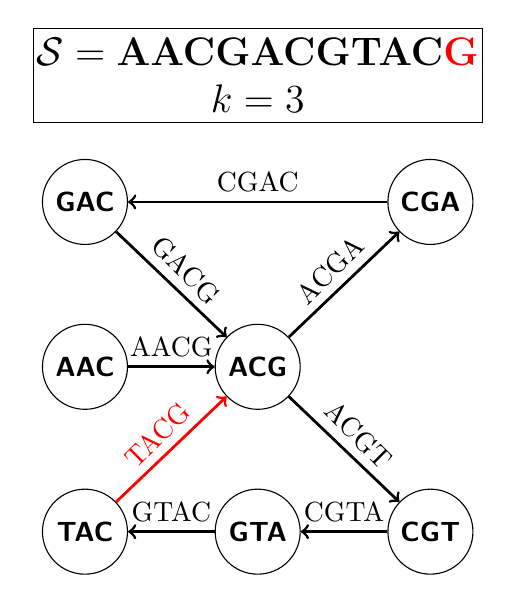
\begin{tikzpicture}	
	\matrix[row sep=10mm,column sep=11mm] {
		\node[kmer](k1){GAC}; & & \node[kmer](k2){CGA}; \\
		\node[kmer](k3){AAC}; & \node[kmer](k4){ACG}; & \\
		\node[kmer](k5){TAC}; &\node[kmer](k7){GTA}; & \node[kmer](k6){CGT}; \\
	};
	\path (k1) edge[->, line width=1] node[above, rotate=-45]{GACG} (k4);
	\path (k2) edge[->, line width=1] node[above]{CGAC} (k1);
	\path (k3) edge[->, line width=1] node[above]{AACG} (k4);
	\path (k4) edge[->, line width=1] node[above, rotate=45]{ACGA} (k2);
	\path (k4) edge[->, line width=1] node[above, rotate=-45]{ACGT} (k6);
	\path (k5) edge[->, color=red, line width=1] node[above, rotate=45, color=red]{TACG} (k4);
	\path (k6) edge[->, line width=1] node[above]{CGTA} (k7);
	\path (k7) edge[->, line width=1] node[above]{GTAC} (k5);
	
	\draw [] (-2.85, 4.3) rectangle (2.85, 3.1);
	\node[font=\Large\bfseries] at (0, 4) {$\mathcal{S} = \mathbf{AACGACGTAC{\color{red} G}}$};
	\node[font=\Large\bfseries] at (0, 3.4) {$k=3$};
	\end{tikzpicture} 
	
\end{document}